\chapter{Energie, Impuls und das elektromagnetische Feld}

Die letzte Vorlesung beginnt mit einer Korrektur und endet bei dem Objekt, das auf der rechten Seite von Einsteins Gleichung stehen wird. Der Weg dorthin ist kein Umweg. Zunächst muss eine Vorzeichenkonvention für das elektrische Feld ausdrücklich festgelegt werden; anschließend müssen drei verschiedene Bedeutungen von Impuls auseinandergehalten werden. Erst nach diesen Vorarbeiten lässt sich die Feldtheorie als gewöhnliche Mechanik mit einem Freiheitsgrad an jedem Raumpunkt lesen. Hamilton-Funktion, lokale Energiedichte, Noether-Impuls, elektromagnetische Energie und Poynting-Vektor ergeben sich dann in einem zusammenhängenden Argument.

\section{Eine Konvention, die konsequent beibehalten werden muss}

Die vorbereitenden Notizen sollten für den Kurs veröffentlicht werden, aber die Frage ist wichtig genug, um sie mündlich zu klären. Byron hatte einen Widerspruch bemerkt – nicht innerhalb der Kursnotation, sondern zwischen dieser Notation und der fast überall sonst verwendeten. Das ist eine Berufsgefahr, wenn man Gleichungen immer wieder neu herleitet: Eine in sich konsistente private Konvention kann von der allgemein üblichen abweichen.

Schreiben wir \(\mathbf E_M\) für die Standardkonvention von Maxwell--Franklin und \(\mathbf E_L\) für die in den vorherigen Vorlesungen verwendete Konvention. Mit der kovarianten Komponente \(A_0\) des Kurses gilt
\begin{align}
\mathbf E_M
  &= -\dot{\mathbf A}+\boldsymbol{\nabla}A_0,
&
\mathbf E_L
  &= +\dot{\mathbf A}-\boldsymbol{\nabla}A_0
   =-\mathbf E_M .
\label{eq:two-electric-conventions}
\end{align}
Viele Bücher führen stattdessen das skalare Potential \(\Phi=-A_0\) ein; dann lautet die erste Formel
\(\mathbf E_M=-\dot{\mathbf A}-\boldsymbol{\nabla}\Phi\).
Das Magnetfeld bleibt unverändert:
\begin{equation}
\mathbf B=\boldsymbol{\nabla}\times\mathbf A.
\label{eq:B-from-A-opening}
\end{equation}

In rationalisierten Einheiten mit \(c=1\) lauten die Standardgleichungen von Maxwell--Franklin
\begin{align}
\boldsymbol{\nabla}\times\mathbf E_M&=-\dot{\mathbf B},
&
\boldsymbol{\nabla}\cdot\mathbf B&=0,
\nonumber\\
\boldsymbol{\nabla}\times\mathbf B&=\dot{\mathbf E}_M+\mathbf J_F,
&
\boldsymbol{\nabla}\cdot\mathbf E_M&=\rho_F .
\label{eq:maxwell-franklin}
\end{align}
Benjamin Franklins historische Wahl legt das Vorzeichen der Ladung fest: In dieser Konvention ist das Elektron negativ. In der Kurskonvention sind auch die Quellenbezeichnungen umgekehrt:
\begin{equation}
\mathbf J_L=-\mathbf J_F,
\qquad
\rho_L=-\rho_F.
\label{eq:source-convention-map}
\end{equation}
Setzt man \(\mathbf E_L=-\mathbf E_M\) ein, erhält man daher
\begin{align}
\boldsymbol{\nabla}\times\mathbf E_L&=+\dot{\mathbf B},
&
\boldsymbol{\nabla}\cdot\mathbf B&=0,
\nonumber\\
\boldsymbol{\nabla}\times\mathbf B&=-\dot{\mathbf E}_L-\mathbf J_L,
&
\boldsymbol{\nabla}\cdot\mathbf E_L&=\rho_L .
\label{eq:maxwell-course-convention}
\end{align}

\begin{figure}[H]\centering

\includegraphics[width=\linewidth]{lecture_10_figure_01.png}\caption{Vollständiger Tafelvergleich zwischen der Maxwell--Franklin- und der Kurskonvention.}\par\smallskip
\textit{Vorlesungsbild: 00:07:10.}\end{figure}

Welche Konvention man verwendet, hat keinen Einfluss auf Messbares. Entscheidend ist die Konsistenz, besonders wenn ein berechnetes Feld mit einem veröffentlichten experimentellen Wert verglichen wird. Der praktische Witz daran ist, dass solche direkten Zahlenvergleiche in der Arbeit des Dozenten so selten vorgekommen waren, dass das entgegengesetzte Vorzeichen unbemerkt blieb, bis der Kurs darauf aufmerksam machte. Für die spätere elektromagnetische Rechnung in diesem Kapitel verwenden wir das Standardfeld \(\mathbf E\equiv\mathbf E_M\).

\section{Drei verschiedene Größen namens Impuls}

Das Wort \emph{Impuls} muss nun genauer aufgeschlüsselt werden. Mechanischer Impuls, kanonischer Impuls und Noether-Impuls können in einfachen Problemen übereinstimmen, aber sie sind keine drei Beschreibungen ein und derselben Größe. In einem allgemeinen System können sie verschiedene Zahlenwerte haben.

\subsection{Mechanischer Impuls}

Für einen Körper mit der Gesamtmasse \(M\) ist der mechanische Impuls
\begin{equation}
\mathbf P_{\mathrm{mech}}=M\dot{\mathbf X}_{\mathrm{cm}}.
\label{eq:mechanical-momentum}
\end{equation}
Für ein einzelnes Teilchen ist \(\mathbf X_{\mathrm{cm}}\) einfach seine Position.
Bei einem zusammengesetzten Körper ist die Einschränkung auf den Schwerpunkt entscheidend.

\begin{figure}[H]\centering
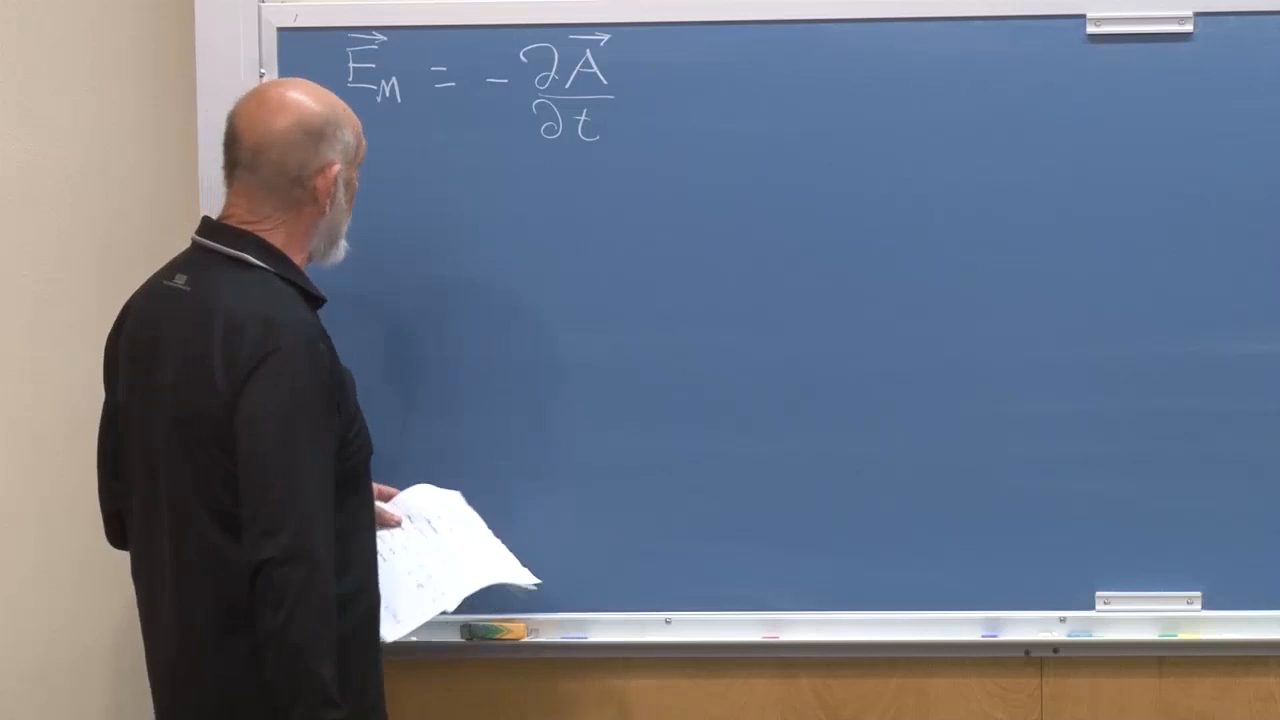
\includegraphics[width=\linewidth]{lecture_10_figure_02.png}\caption{Einführung des mechanischen Impulses als Masse mal Schwerpunktgeschwindigkeit.}\par\smallskip
\textit{Vorlesungsbild: 00:11:15.}\end{figure}

\subsection{Kanonischer Impuls}

Angenommen, die Mechanik wird beschrieben durch
\(L(q_i,\dot q_i)\). Der zu \(q_i\) kanonisch konjugierte Impuls ist
\begin{equation}
p_i=\frac{\partial L}{\partial\dot q_i}.
\label{eq:canonical-momentum}
\end{equation}
Für
\begin{equation}
L=\frac12 m\dot{\mathbf x}^{\,2}-V(\mathbf x),
\label{eq:simple-particle-lagrangian}
\end{equation}
ergibt sich damit \(\mathbf p=m\dot{\mathbf x}\); kanonischer und mechanischer Impuls stimmen hier also zufällig überein.

\begin{figure}[H]\centering
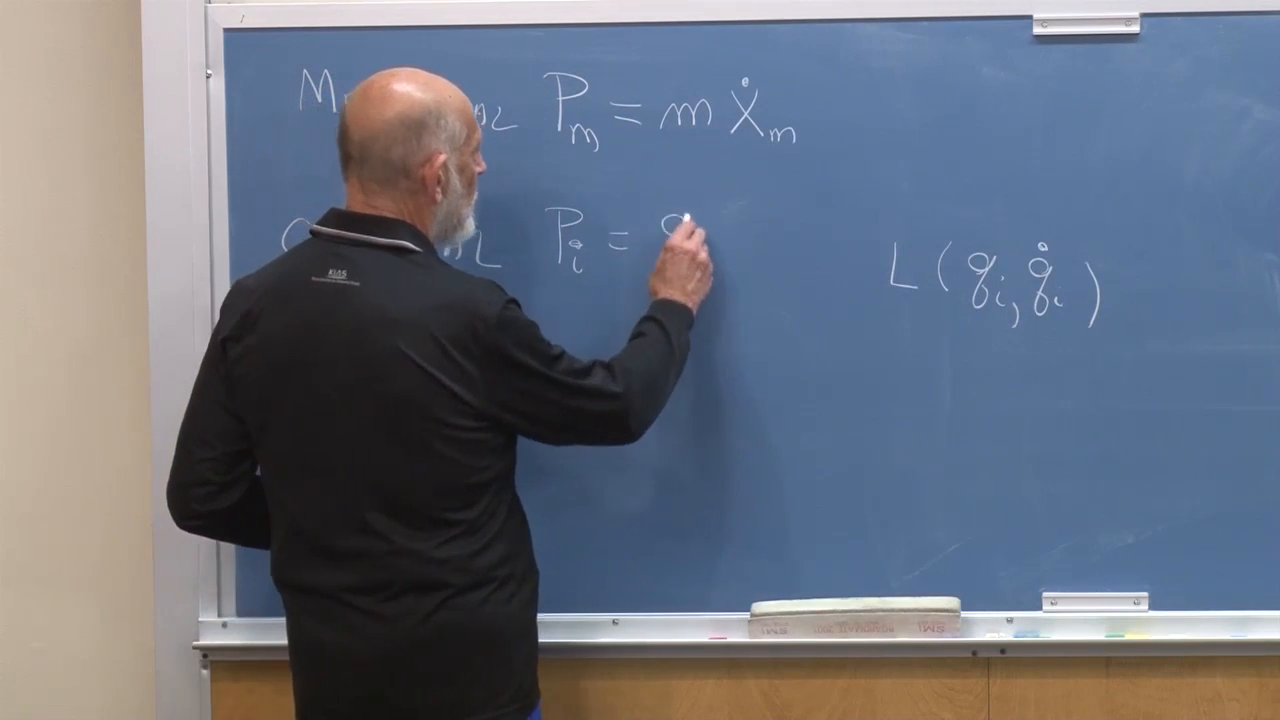
\includegraphics[width=\linewidth]{lecture_10_figure_03.png}\caption{Mechanischer und kanonischer Impuls neben der einfachen Teilchen-Lagrange-Funktion.}\par\smallskip
\textit{Vorlesungsbild: 00:13:40.}\end{figure}

Ein geladenes Teilchen in einem Magnetfeld ist das nützliche Gegenbeispiel. Mit der an der Tafel angegebenen Vorzeichenkonvention gilt
\begin{equation}
L=\frac12m\dot{\mathbf x}^{\,2}-V(\mathbf x)
  -e\,\dot{\mathbf x}\cdot\mathbf A(\mathbf x),
\label{eq:magnetic-particle-lagrangian}
\end{equation}
und daher
\begin{equation}
p_i=m\dot x_i-eA_i.
\label{eq:magnetic-canonical-shift}
\end{equation}
Eine Änderung der Ladungskonvention oder des Vorzeichens des Wechselwirkungsterms ändert das angezeigte Vorzeichen, nicht aber die Lehre: Der kanonische Impuls enthält einen Beitrag des Vektorpotentials und ist nicht einfach \(m\dot x_i\). Hamilton-Gleichungen verwenden die kanonische Variable. Später kann man den feldabhängigen Term auf die andere Seite einer Gleichung bringen und so eine Newton ähnlich sehende Beschleunigungsgleichung erhalten; diese Umformung ändert jedoch nicht die Definition.

\begin{figure}[H]\centering
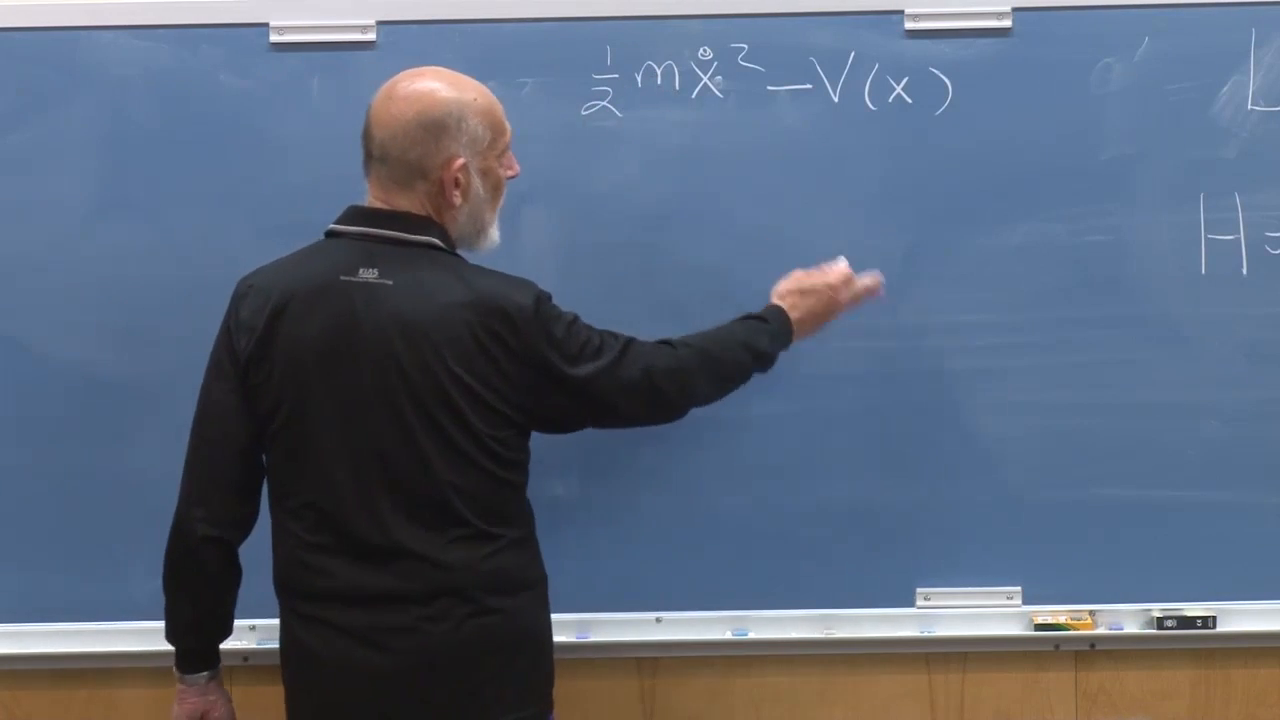
\includegraphics[width=\linewidth]{lecture_10_figure_04.png}\caption{Der Beitrag des Vektorpotentials verschiebt den kanonischen Impuls gegenüber dem mechanischen Impuls.}\par\smallskip
\textit{Vorlesungsbild: 00:15:50.}\end{figure}

\subsection{Noether-Impuls}

Der dritte Impuls ist die erhaltene Ladung, die mit der Invarianz unter räumlichen Translationen verbunden ist. Für eine infinitesimale Symmetrie
\begin{equation}
q_i\longrightarrow q_i+\delta q_i
\end{equation}
die die Lagrange-Funktion invariant lässt, ergibt der Noether-Satz bis auf die Normierung des infinitesimalen Parameters
\begin{equation}
Q=\sum_i p_i\,\delta q_i.
\label{eq:noether-charge-mechanics}
\end{equation}
Die hier auftretenden \(p_i\) sind kanonische Impulse. Ist die Symmetrie eine gleichförmige Translation und stimmt der kanonische Impuls zufällig mit dem mechanischen Impuls überein, dann ergibt sich aus \(Q\) der bekannte Gesamtimpuls. In einem weniger einfachen System muss diese Übereinstimmung bewiesen werden; man darf sie nicht voraussetzen.

\begin{figure}[H]\centering
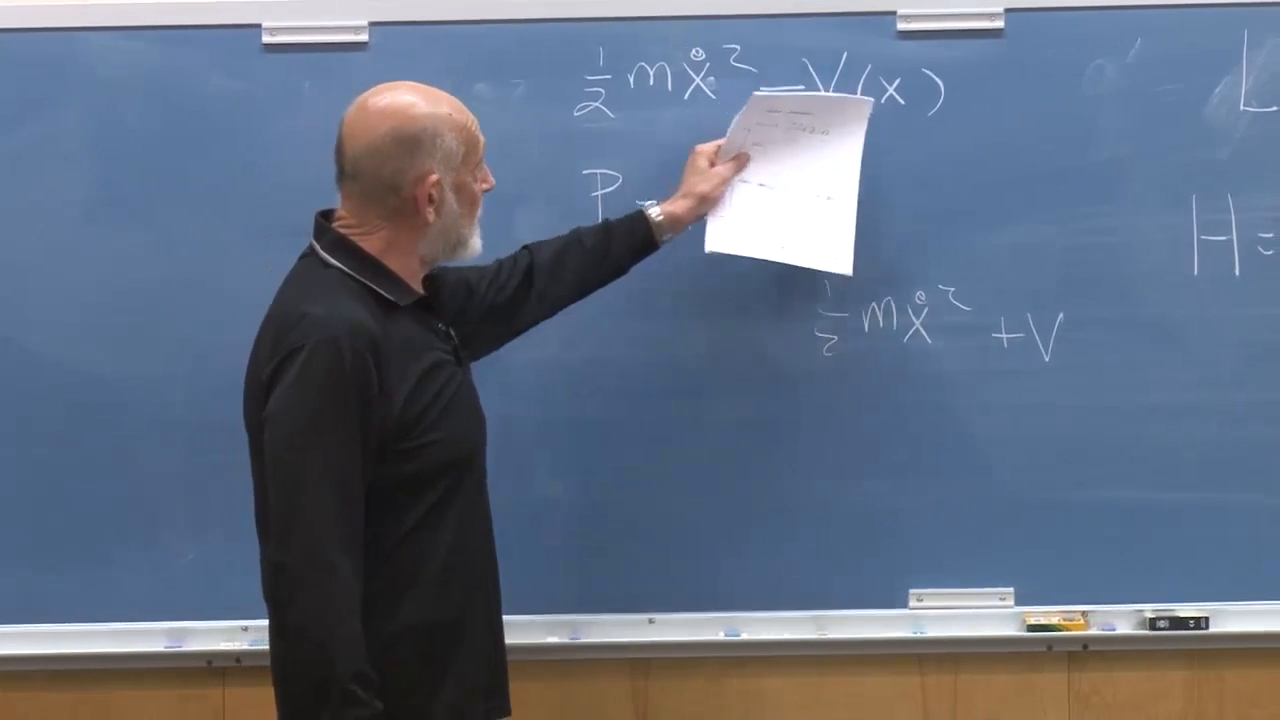
\includegraphics[width=\linewidth]{lecture_10_figure_05.png}\caption{Die Noether-Ladung, zusammengesetzt aus kanonischen Impulsen und den infinitesimalen Änderungen der Koordinaten.}\par\smallskip
\textit{Vorlesungsbild: 00:19:00.}\end{figure}

\section{Energie als Hamilton-Funktion}

Räumliche Translationen führen zum Impuls, zeitliche Translationen zur Energie. Hängt die Lagrange-Funktion nicht explizit von der Zeit ab, so ist die Hamilton-Funktion
\begin{equation}
H=\sum_i p_i\dot q_i-L
\label{eq:hamiltonian-definition}
\end{equation}
erhalten. Sie ist die Legendre-Transformation der Lagrange-Funktion und keine Regel, nach der man Vorzeichen durch bloßes Hinsehen ändert.

\begin{figure}[H]\centering
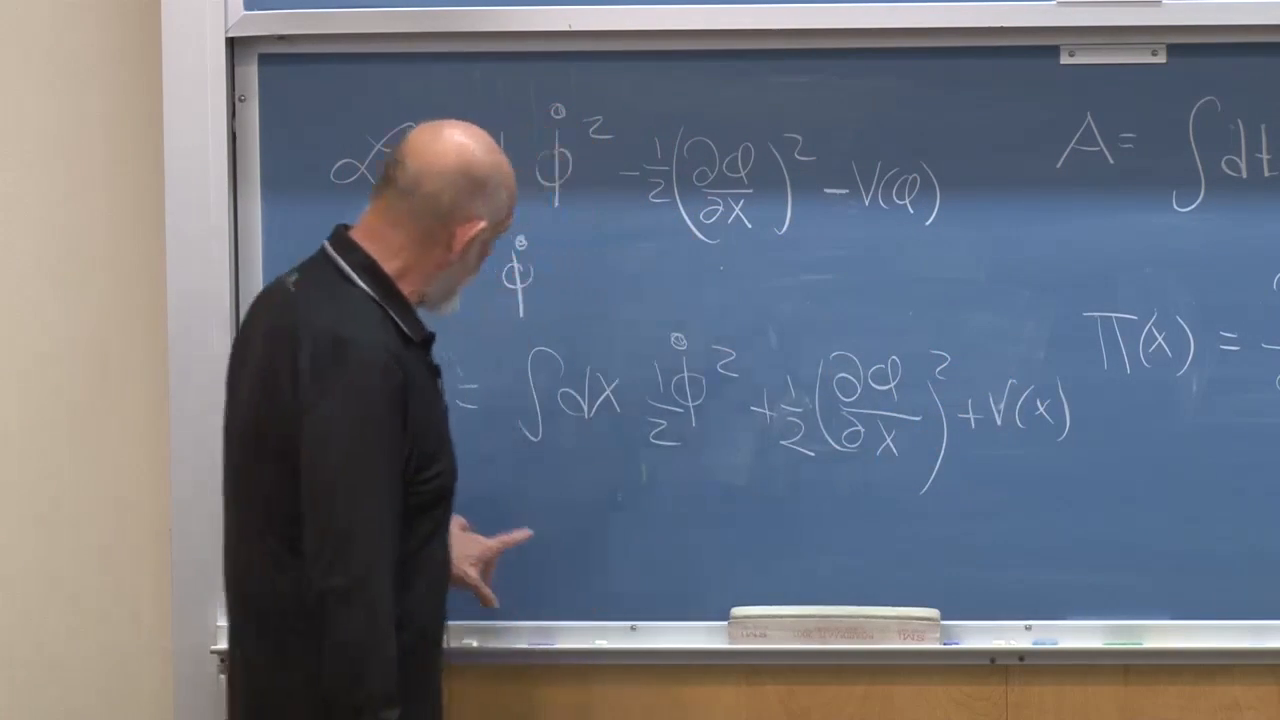
\includegraphics[width=\linewidth]{lecture_10_figure_06.png}\caption{Die Hamilton-Funktion als Legendre-Transformation einer allgemeinen Lagrange-Funktion.}\par\smallskip
\textit{Vorlesungsbild: 00:22:55.}\end{figure}

Für das Beispiel mit einem Teilchen gilt
\begin{align}
p&=m\dot x,
\nonumber\\
H&=p\dot x-L\\
&=m\dot x^2
  -\left(\frac12m\dot x^2-V(x)\right)\\
&=\frac12m\dot x^2+V(x).
\label{eq:particle-hamiltonian}
\end{align}
Die Lagrange-Funktion ist also kinetische minus potenzielle Energie, während die Hamilton-Funktion kinetische plus potenzielle Energie ist.

\begin{figure}[H]\centering
\includegraphics[width=\linewidth]{lecture_10_figure_07.png}\caption{Die Teilchenrechnung zeigt, wie \(H=T+V\) aus \(H=p\dot x-L\) folgt.}\par\smallskip
\textit{Vorlesungsbild: 00:24:20.}\end{figure}

Wenn jede Geschwindigkeitsabhängigkeit ein übliches positives quadratisches kinetisches Glied ist und der übrige Teil keine Geschwindigkeiten enthält, lässt sich die Hamilton-Funktion direkt ablesen, indem man das Vorzeichen des geschwindigkeitsunabhängigen Teils umkehrt. Diese Abkürzung werden wir wiederholt verwenden. Sie ist nur deshalb zulässig, weil die Legendre-Transformation in den betrachteten Beispielen diese einfache Form hat.

\section{Ein Feld ist ein mechanisches System mit unendlich vielen Koordinaten}

Um die mechanische Struktur der Feldtheorie sichtbar zu machen, wählen wir ein Inertialsystem und bestehen vorübergehend nicht darauf, dass jede Zeile manifest Lorentz-kovariant ist. Die klassische Mechanik hat eine Zeitachse und Koordinaten \(q_i(t)\). Ein Skalarfeld hat eine Zeitachse und Koordinaten \(\phi(\mathbf x,t)\). Die diskrete Bezeichnung \(i\) ist einfach zur kontinuierlichen Bezeichnung \(\mathbf x\) geworden:
\begin{equation}
q_i(t)\quad\longrightarrow\quad\phi(\mathbf x,t).
\label{eq:discrete-to-field}
\end{equation}
Der Feldwert an jedem Raumpunkt ist ein Freiheitsgrad. Hier bezeichnet \(\mathbf x\), welcher Freiheitsgrad gemeint ist; die Ortskoordinate ist nicht selbst die verallgemeinerte Koordinate.

\begin{figure}[H]\centering
\includegraphics[width=\linewidth]{lecture_10_figure_08.png}\caption{Ein räumliches Gitter, auf dem der Feldwert an jedem Punkt als eigener mechanischer Freiheitsgrad dargestellt wird.}\par\smallskip
\textit{Vorlesungsbild: 00:30:15.}\end{figure}

\begin{classroomqa}\audiencequestion{Warum schreiben wir das Feld nicht gleich als \(\phi(\mathbf x,t)\)?}\lecturerresponse{Das ist die vollständige Notation. Die vorübergehende Schreibweise \(\phi(\mathbf x)\) lässt das gemeinsame Zeitargument weg, so wie man oft \(q_i\) schreibt und dabei im Kopf behält, dass jedes \(q_i\) von der Zeit abhängt. Die Bezeichnung \(i\) oder nun \(\mathbf x\) gibt an, welcher Freiheitsgrad betrachtet wird. \lecturetimestamp{00:32:43}}\end{classroomqa}

\begin{classroomqa}\audiencequestion{Sind die Feldwerte an benachbarten Punkten wirklich unabhängige Koordinaten? Was erzwingt ihre Stetigkeit?}\lecturerresponse{Sie sind unabhängige kanonische Koordinaten. Glattheit wird nicht dadurch erzwungen, dass benachbarte Werte gleichgesetzt werden; sie ergibt sich dynamisch. Die Hamilton-Funktion enthält ein positives Gradientenenergieglied. Daher kostet ein fester Sprung über eine immer kleinere Entfernung immer mehr Energie. Konfigurationen endlicher Energie sind im Kontinuumslimes folglich glatt. \lecturetimestamp{00:33:09}}\end{classroomqa}

Eine räumliche Ableitung macht die Kopplung benachbarter Freiheitsgrade explizit. Auf einem Gitter mit Gitterabstand \(\epsilon\) gilt
\begin{equation}
\partial_x\phi(x,t)
  =\lim_{\epsilon\to0}
   \frac{\phi(x+\epsilon,t)-\phi(x,t)}{\epsilon}.
\label{eq:field-finite-difference}
\end{equation}
Sie hängt von zwei benachbarten Koordinaten ab, enthält aber keine verallgemeinerte Geschwindigkeit. In der mechanischen Analogie gehört sie zur Koordinatenabhängigkeit der Lagrange-Funktion, nicht zur Abhängigkeit von \(\dot q_i\).

\begin{figure}[H]\centering
\includegraphics[width=\linewidth]{lecture_10_figure_09.png}\caption{Die räumliche Ableitung, rekonstruiert als Differenz benachbarter Feldwerte auf dem Gitter.}\par\smallskip
\textit{Vorlesungsbild: 00:31:40.}\end{figure}

Die Wirkung lässt sich nun in ausdrücklich mechanischer Form schreiben:
\begin{align}
S&=\int dt\,L,
\nonumber\\
L&=\int d^3x\,
\mathcal L\!\left(
\phi,\dot\phi,\boldsymbol{\nabla}\phi
\right),
\nonumber\\
S&=\int dt\,d^3x\,
\mathcal L\!\left(
\phi,\dot\phi,\boldsymbol{\nabla}\phi
\right).
\label{eq:field-action-split}
\end{align}
Der kalligrafische Buchstabe \(\mathcal L\) bezeichnet die Lagrange-Dichte; ihre Integration über den Raum ergibt die gewöhnliche Lagrange-Funktion, die über die Zeit integriert wird. Eine lokale Theorie koppelt jeden Punkt nur über die Felder und ihre Ableitungen an diesem Punkt. Die Aufspaltung von Zeit und Raum verbirgt vorübergehend die Lorentz-Kovarianz, macht aber die mechanische Struktur durchsichtig.

\begin{figure}[H]\centering
\includegraphics[width=\linewidth]{lecture_10_figure_10.png}\caption{Die Feldwirkung, aufgeteilt in ein Zeitintegral und ein Raumintegral über die Lagrange-Dichte.}\par\smallskip
\textit{Vorlesungsbild: 00:36:40.}\end{figure}

\section{Kanonischer Feldimpuls und Hamilton-Dichte}

Die Geschwindigkeit einer Feldkoordinate ist \(\dot\phi(\mathbf x,t)\): Sie gibt an, wie sich das Feld mit der Zeit an einem festen Punkt ändert. Sie beschreibt keine Bewegung von einem Raumpunkt zu einem anderen. Der zum Feld kanonisch konjugierte Impuls ist daher selbst ein Feld:
\begin{equation}
\Pi(\mathbf x,t)
 =\frac{\partial\mathcal L}{\partial\dot\phi(\mathbf x,t)}.
\label{eq:field-canonical-momentum}
\end{equation}
Bei mehreren Feldern \(\phi_a\) gibt es für jedes davon ein Impulsfeld \(\Pi_a\).

In der Legendre-Transformation wird die diskrete Summe durch ein Raumintegral ersetzt:
\begin{align}
H
 &=\int d^3x\,
   \left[\Pi\dot\phi-\mathcal L\right]
  =\int d^3x\,\mathcal H,
\nonumber\\
\mathcal H
 &=\Pi\dot\phi-\mathcal L .
\label{eq:field-hamiltonian-density}
\end{align}
Die Größe im Integranden ist die Energiedichte.

\begin{figure}[H]\centering
\includegraphics[width=\linewidth]{lecture_10_figure_11.png}\caption{Die Legendre-Transformation für Felder und ihre Deutung als Integral der lokalen Energiedichte.}\par\smallskip
\textit{Vorlesungsbild: 00:42:40.}\end{figure}

\begin{classroomqa}\audiencequestion{Warum darf die Ableitung der gesamten Lagrange-Funktion nach \(\dot\phi\) an einem Punkt durch die Ableitung der lokalen Dichte dort ersetzt werden?}\lecturerresponse{Man kann sich das Raumintegral als kontinuierliche Summe vorstellen. Unter der hier verwendeten Lokalitätsannahme tritt die Geschwindigkeit \(\dot\phi(\mathbf x)\) nur in dem Term auf, der zu eben diesem Punkt gehört. Die Ableitung nach genau dieser Geschwindigkeit lässt alle anderen Terme wegfallen. Räumliche Ableitungen können benachbarte Feldwerte koppeln, führen in dieser Theorie aber keine benachbarten Zeitableitungen ein. \lecturetimestamp{00:51:56}}\end{classroomqa}

\subsection{Das Skalarfeld}

Betrachten wir eine Raumdimension und setzen
\begin{equation}
\mathcal L
 =\frac12\dot\phi^2
  -\frac12(\partial_x\phi)^2
  -V(\phi).
\label{eq:scalar-field-lagrangian}
\end{equation}
Dies ist die nichtkovariante Darstellung des zuvor verwendeten Lorentz-Skalars: Das relative Minuszeichen zwischen zeitlichen und räumlichen Ableitungen stammt von der Minkowski-Metrik. Der kanonische Impuls ist
\begin{equation}
\Pi=\dot\phi,
\label{eq:scalar-pi}
\end{equation}
und die Hamilton-Funktion lautet
\begin{equation}
H=\int dx\,
\left[
\frac12\dot\phi^2
+\frac12(\partial_x\phi)^2
+V(\phi)
\right].
\label{eq:scalar-field-hamiltonian}
\end{equation}
Während der Rechnung wurde das Potential vorübergehend als \(V(x)\) bezeichnet; der Kurs korrigierte die Bezeichnung zu \(V(\phi)\). Es kann indirekt über das Feld von der Position abhängen, hat in der translationsinvarianten Theorie aber keine vorgegebene äußere Abhängigkeit von \(x\).

\begin{figure}[H]\centering
\includegraphics[width=\linewidth]{lecture_10_figure_12.png}\caption{Skalarfeld-Lagrange-Dichte, konjugierter Impuls und positive Hamilton-Funktion, gemeinsam an der Tafel zusammengestellt.}\par\smallskip
\textit{Vorlesungsbild: 00:47:05.}\end{figure}

Der gesamte Anteil ohne Zeitableitungen spielt die Rolle der potenziellen Energie. Dazu gehören sowohl \(V(\phi)\) als auch die Gradientenenergie \(\frac12(\partial_x\phi)^2\). Die Lagrange-Funktion kann positiv oder negativ sein; eine stabile Energie sollte nach unten beschränkt sein.

\begin{classroomqa}\audiencequestion{Darf das Potential \(V(\phi)\) negativ sein?}\lecturerresponse{Ja. Ist es nach unten beschränkt, kann man eine Konstante addieren, sodass sein Minimum null ist, ohne die klassische Feldgleichung zu ändern. Ein nach unten unbeschränktes Potential beschreibt eine Instabilität: Das Feld kann seine Energie unbegrenzt senken. Das stabile Vakuum ist ein konstantes Feld, das an einem Minimum des verschobenen Potentials liegt. \lecturetimestamp{00:49:03}}\end{classroomqa}

Die frühere Frage nach der Stetigkeit lässt sich nun quantitativ beantworten. Ein Sprung \(\Delta\phi\) über einen Gitterabstand \(\epsilon\) trägt bei
\begin{equation}
\frac12(\partial_x\phi)^2
\sim\frac12\left(\frac{\Delta\phi}{\epsilon}\right)^2.
\label{eq:gradient-cost}
\end{equation}
Für \(\epsilon\to0\) ergibt ein fester Sprung eine beliebig große Energiedichte. Konfigurationen mit starken Unstetigkeiten werden daher durch die endliche Energie unterdrückt.

\begin{figure}[H]\centering
\includegraphics[width=\linewidth]{lecture_10_figure_13.png}\caption{Die Skalarfeld-Energieformel bleibt stehen, während die Skizze an der Tafel ein glattes Feld einer abrupten Änderung gegenüberstellt.}\par\smallskip
\textit{Vorlesungsbild: 00:54:20.}\end{figure}

\section{Lokale Energie und die Bedeutung von \texorpdfstring{\(T^{00}\)}{T00}}

Die Energiedichte erhält eine kompakte Bezeichnung:
\begin{equation}
T^{00}=\mathcal H=\Pi\dot\phi-\mathcal L.
\label{eq:T00-definition}
\end{equation}
Die beiden Nullindizes drücken zwei verschiedene Aussagen aus. Energie ist die Zeitkomponente \(P^0\) des Energie--Impuls-Vierervektors, während eine Dichte die Zeitkomponente eines Erhaltungsstroms ist. Somit ist \(T^{00}\) die Dichte der Zeitkomponente des Viererimpulses.

\begin{figure}[H]\centering
\includegraphics[width=\linewidth]{lecture_10_figure_14.png}\caption{Das Feldenergie-Integral wird lokal geschrieben und mit \(T^{00}\) identifiziert.}\par\smallskip
\textit{Vorlesungsbild: 01:00:00.}\end{figure}

Erhaltung in einer relativistischen lokalen Theorie bedeutet mehr, als dass eine globale Zahl unverändert bleibt. Energie kann nicht im Labor verschwinden und bei Alpha Centauri wieder auftauchen. Eine Änderung innerhalb eines Gebiets muss durch einen Fluss über dessen Rand erklärt werden. In lokaler Form gilt
\begin{equation}
\partial_\mu T^{\mu\nu}=0,
\label{eq:stress-energy-continuity}
\end{equation}
Der erste Index bezeichnet also die Dichte oder die Flussrichtung, der zweite gibt an, welche Komponente \(P^\nu\) transportiert wird.

\begin{classroomqa}\audiencequestion{Bedeutet die Bezeichnung \(T^{00}\) als Dichte, dass man die Gesamtenergie durch Integration darüber erhält?}\lecturerresponse{Genau:
\(E=P^0=\int d^3x\,T^{00}\). Die lokale Dichte steht als Integrand in der Legendre-Transformation des Feldes. Eine Änderung an einem Ort wird durch einen Energiestrom zwischen benachbarten Orten ausgeglichen. \lecturetimestamp{00:59:06}}\end{classroomqa}

\section{Impulsdichte aus räumlichen Translationen}

Kehren wir zur Noether-Formel zurück und ersetzen nun die diskrete Summe durch ein Raumintegral. Bei einer kleinen Translation in \(m\)-Richtung ändert sich das Feld gemäß
\begin{equation}
\delta\phi
  =\phi(\mathbf x)-\phi(\mathbf x-\boldsymbol{\epsilon})
  =\epsilon^m\partial_m\phi+O(\epsilon^2),
\label{eq:translated-field-change}
\end{equation}
für die an der Tafel verwendete passive Konvention. Bei einem Wechsel zwischen aktiven und passiven Translationen kehrt sich das Gesamtvorzeichen um; sobald diese Konvention festgelegt ist, steht auch der physikalische Erzeuger fest. Klammert man \(\epsilon^m\) aus, hat der Noether-Impuls die Form
\begin{equation}
P_m\ \propto\ \int d^3x\,\Pi\,\partial_m\phi.
\label{eq:scalar-noether-momentum}
\end{equation}

\begin{figure}[H]\centering
\includegraphics[width=\linewidth]{lecture_10_figure_15.png}\caption{Ein verschobenes Feldprofil und die Ableitung, die seine infinitesimale Änderung misst.}\par\smallskip
\textit{Vorlesungsbild: 01:04:20.}\end{figure}

\begin{classroomqa}\audiencequestion{Warum blieb die infinitesimale Translation \(\epsilon\) nicht in der Impulsformel stehen?}\lecturerresponse{Die Noether-Ladung ergibt sich zunächst proportional zu \(\epsilon\). Der Impuls ist als Koeffizient dieses beliebigen Translationsparameters definiert, daher wird \(\epsilon\) herausgekürzt. Eine erhaltene Größe mit einer festen Konstante zu multiplizieren, würde an ihrer Erhaltung nichts ändern; durch das Herausziehen des Koeffizienten erhält man jedoch die übliche Normierung. \lecturetimestamp{01:04:45}}\end{classroomqa}

\begin{classroomqa}\audiencequestion{Wird das Translationsintervall im Kontinuumsintegral zu \(dx\)?}\lecturerresponse{Sie stammen aus unterschiedlichen Grenzübergängen. Das Maß \(dx\) ergibt sich, wenn die Summe über räumlich bezeichnete Freiheitsgrade durch ein Integral ersetzt wird. Der Translationsparameter \(\epsilon\) beschreibt die Symmetrieoperation und wird aus ihrer Noether-Ladung ausgeklammert. In der Zwischenrechnung sind beide infinitesimal, erfüllen aber unterschiedliche Aufgaben. \lecturetimestamp{01:05:16}}\end{classroomqa}

In der Notation der Vorlesung lautet die Dichte der \(m\)-Komponente des Impulses
\begin{equation}
T^{0m}=\Pi\,\partial_m\phi,
\label{eq:scalar-momentum-density}
\end{equation}
bei vorausgesetzter Vorzeichenkonvention für Translationen. Für die Skalarfeldtheorie gilt \(\Pi=\dot\phi\), sodass sie proportional zu \(\dot\phi\,\partial_m\phi\) ist.

\begin{figure}[H]\centering
\includegraphics[width=\linewidth]{lecture_10_figure_16.png}\caption{Die Noether-Impulsdichte \(T^{0m}=\Pi\,\partial_m\phi\) an der Tafel.}\par\smallskip
\textit{Vorlesungsbild: 01:07:10.}\end{figure}

Das ist ein Impuls, den eine Welle tatsächlich trägt. Translationsinvarianz gilt nur, wenn alles verschoben wird: Felder, Teilchen, Quellen und Apparaturen. Wird ein Lichtpuls von einer frei aufgehängten Platte absorbiert, erhält die Platte einen Rückstoß. Bei gewöhnlichem Licht ist der Effekt winzig; ein ausreichend leistungsstarker Laser kann jedoch genügend Impuls übertragen, um ein kleines Ziel zu komprimieren. Der erhaltene Gesamtimpuls gehört den Teilchen und den Feldern gemeinsam.

\subsection{Was tritt an die Stelle der Newton-Gleichung?}

Die aus ~\eqref{eq:scalar-field-lagrangian} hergeleitete Euler--Lagrange-Gleichung für das Feld lautet
\begin{equation}
\ddot\phi-\nabla^2\phi=-\frac{dV}{d\phi}.
\label{eq:scalar-equation-of-motion}
\end{equation}
Sie ist das Analogon des Newtonschen Gesetzes in der Feldtheorie.

\begin{figure}[H]\centering
\includegraphics[width=\linewidth]{lecture_10_figure_17.png}\caption{Die Skalarfeldgleichung neben ihrer Hamilton-Funktion und Impulsdichte.}\par\smallskip
\textit{Vorlesungsbild: 01:12:55.}\end{figure}

\begin{classroomqa}\audiencequestion{Was entspricht dem Newtonschen Gesetz für ein Feld?}\lecturerresponse{Das leistet die Euler--Lagrange-Gleichung für das Feld. Hier ist sie eine Wellengleichung mit dem Kraftterm \(-V'(\phi)\). Die Rolle von \(m\ddot x=-V'(x)\) übernimmt \(\ddot\phi-\nabla^2\phi=-V'(\phi)\). \lecturetimestamp{01:11:48}}\end{classroomqa}

\begin{classroomqa}\audiencequestion{Woher wissen wir, ob eine vorgeschlagene Feld-Lagrange-Funktion richtig ist? Müssen wir die Feldgleichung bereits kennen?}\lecturerresponse{Beide Richtungen sind möglich. Historisch kann man aus Experimenten Gleichungen erschließen und anschließend nach einer Wirkung suchen, wie es bei Newton und Maxwell geschah. In der modernen Theorie geht man oft vom Feldinhalt, der Lokalität, der Symmetrie und einer kleinen Menge zulässiger Terme aus, leitet daraus die Gleichungen her und prüft ihre Vorhersagen. Das dargestellte Skalarfeld könnte ein fundamentales Feld beschreiben, aber ebenso die Querverschiebung eines Seils, dessen Kontinuumswirkung aus seinen Teilchen hergeleitet wird. \lecturetimestamp{01:12:55}}\end{classroomqa}

\section{Das elektromagnetische Feld in zeitlicher Eichung}

Die bereits gefundenen Komponenten \(T^{00}\) und \(T^{0m}\) gehören zum Energie--Impuls-Tensor. Seine übrigen Komponenten beschreiben Energie- und Impulsflüsse. Dieser Tensor wird später als Quelle der Gravitation dienen; das unmittelbare Beispiel liefert jedoch der Elektromagnetismus.

Die grundlegende elektromagnetische Koordinate ist das Viererpotential \(A_\mu\). Die Eichfreiheit erlaubt die Transformation
\begin{equation}
A_\mu\longrightarrow A'_\mu=A_\mu+\partial_\mu S
\label{eq:gauge-transformation-lecture10}
\end{equation}
ohne \(F_{\mu\nu}\) zu ändern. Wählen wir \(S\) so, dass
\begin{equation}
\partial_tS=-A_0.
\label{eq:temporal-gauge-choice}
\end{equation}
Zum Beispiel kann man \(A_0\) an jedem festen Raumpunkt über die Zeit integrieren. Dann verschwindet die transformierte Zeitkomponente:
\begin{equation}
A'_0=A_0+\partial_tS=0.
\label{eq:temporal-gauge}
\end{equation}
Das ist die zeitliche Eichung. Sie entfernt \(A_0\) aus der Menge der dynamischen Koordinaten, doch das Gaußsche Gesetz bleibt als Zwangsbedingung bestehen, ebenso eine zeitunabhängige Resteichfreiheit.

\begin{figure}[H]\centering
\includegraphics[width=\linewidth]{lecture_10_figure_18.png}\caption{Die Eichfreiheit wird genutzt, um \(A_0=0\) durch Lösung von \(\partial_tS=-A_0\) zu wählen.}\par\smallskip
\textit{Vorlesungsbild: 01:20:15.}\end{figure}

Von jetzt an bezeichne \(\mathbf E\) das Standardfeld von Maxwell. Vor der Eichfixierung gilt
\begin{equation}
E_m=-\partial_tA_m+\partial_mA_0,
\qquad
\mathbf B=\boldsymbol{\nabla}\times\mathbf A.
\label{eq:E-B-general-potential}
\end{equation}
In zeitlicher Eichung vereinfacht sich dies zu
\begin{equation}
\mathbf E=-\dot{\mathbf A},
\qquad
\mathbf B=\boldsymbol{\nabla}\times\mathbf A.
\label{eq:E-B-temporal-gauge}
\end{equation}
Zeitableitungen von \(\mathbf A\) ergeben das elektrische Feld; räumliche Ableitungen ergeben das Magnetfeld.

\begin{figure}[H]\centering
\includegraphics[width=\linewidth]{lecture_10_figure_19.png}\caption{Elektrisches und magnetisches Feld in zeitlicher Eichung: \(\mathbf E=-\dot{\mathbf A}\) und \(\mathbf B=\nabla\times\mathbf A\).}\par\smallskip
\textit{Vorlesungsbild: 01:23:50.}\end{figure}

\section{Kanonischer Impuls und Energie des elektromagnetischen Feldes}

Die freie Lagrange-Dichte von Maxwell lautet
\begin{equation}
\mathcal L_{\mathrm{EM}}
 =-\frac14F_{\mu\nu}F^{\mu\nu}
 =\frac12\left(\mathbf E^2-\mathbf B^2\right).
\label{eq:maxwell-lagrangian-energy-lecture}
\end{equation}
In zeitlicher Eichung gilt
\begin{equation}
\mathcal L_{\mathrm{EM}}
 =\frac12\dot{\mathbf A}^{\,2}
  -\frac12(\boldsymbol{\nabla}\times\mathbf A)^2.
\label{eq:maxwell-lagrangian-temporal}
\end{equation}
Sie hat genau die Form des Skalarfelds: Quadrate der Zeitableitungen minus Quadrate der räumlichen Ableitungen.

\begin{figure}[H]\centering
\includegraphics[width=\linewidth]{lecture_10_figure_20.png}\caption{Die Lagrange-Funktion von Maxwell, umgeschrieben als mechanische Feld-Lagrange-Funktion für die räumlichen Komponenten von \(\mathbf A\).}\par\smallskip
\textit{Vorlesungsbild: 01:28:10.}\end{figure}

Zu jeder Komponente \(A_m\) gehört ein kanonischer Impuls:
\begin{equation}
\Pi_m
 =\frac{\partial\mathcal L_{\mathrm{EM}}}
        {\partial\dot A_m}
 =\dot A_m
 =-E_m.
\label{eq:em-canonical-momentum}
\end{equation}
Das ist ein konkretes Beispiel dafür, warum die Konvention wichtig ist. Bei der zuvor verwendeten entgegengesetzten Konvention für das elektrische Feld würde sich das Vorzeichen in der letzten dargestellten Gleichung ändern, die kanonische Ableitung selbst jedoch nicht.

\begin{figure}[H]\centering
\includegraphics[width=\linewidth]{lecture_10_figure_21.png}\caption{Die drei kanonischen Impulsfelder zu \(A_x,A_y,A_z\) sind jeweils gleich der entsprechenden Zeitableitung und damit gleich dem negativen Standard-Elektrofeld.}\par\smallskip
\textit{Vorlesungsbild: 01:30:20.}\end{figure}

Die Abkürzung für die Hamilton-Funktion ist nun begründet: Man kehrt das Vorzeichen des Terms ohne Zeitableitungen um. Die elektromagnetische Energiedichte ist
\begin{equation}
T^{00}_{\mathrm{EM}}
 =\mathcal H_{\mathrm{EM}}
 =\frac12\left(\mathbf E^2+\mathbf B^2\right),
\label{eq:em-energy-density}
\end{equation}
und die Gesamtenergie lautet
\begin{equation}
H_{\mathrm{EM}}
 =\int d^3x\,
\frac12\left(\mathbf E^2+\mathbf B^2\right).
\label{eq:em-total-energy}
\end{equation}
Anders als die Lagrange-Dichte ist die Energiedichte nichtnegativ.

\begin{figure}[H]\centering
\includegraphics[width=\linewidth]{lecture_10_figure_22.png}\caption{Die positive elektromagnetische Hamilton-Dichte \(\frac12(\mathbf E^2+\mathbf B^2)\).}\par\smallskip
\textit{Vorlesungsbild: 01:32:00.}\end{figure}

Für eine ebene Welle im Vakuum gilt \(\mathbf E\perp\mathbf B\); die beiden Felder sind phasengleich und haben in Einheiten mit \(c=1\) den gleichen Betrag. Daher tragen das elektrische und das magnetische Feld jeweils gleich viel zur Wellenenergie bei:
\begin{equation}
u_E=\frac12\mathbf E^2,
\qquad
u_B=\frac12\mathbf B^2,
\qquad
u_E=u_B.
\label{eq:plane-wave-energy-halves}
\end{equation}

\section{Herleitung des elektromagnetischen Impulses}

Die Noether-Formel für Translationen muss nun über die drei Felder \(A_m\) summiert werden. Wählt man das Vorzeichen der Translation so, dass der physikalische Impuls in Ausbreitungsrichtung zeigt, lautet die \(n\)-Komponente
\begin{equation}
P_n
 =\int d^3x\,E_m\,\partial_nA_m,
\label{eq:em-canonical-noether-momentum}
\end{equation}
wobei über \(m\) summiert wird. Die Vorlesung hält ausdrücklich beim Vorzeichen inne: Es hängt von den zuvor gewählten Konventionen für das elektrische Feld sowie für aktive und passive Translationen ab. Das eichinvariante physikalische Ergebnis wird das Vorzeichen festlegen.

\begin{figure}[H]\centering
\includegraphics[width=\linewidth]{lecture_10_figure_23.png}\caption{Die Noether-Formel für das Skalarfeld, erweitert auf die drei Komponenten des Vektorpotentials.}\par\smallskip
\textit{Vorlesungsbild: 01:36:40.}\end{figure}

Der Integrand enthält nach wie vor das Eichpotential und nicht nur die physikalischen Felder. Addiert und subtrahiert man \(E_m\partial_mA_n\), erhält man:
\begin{align}
E_m\partial_nA_m
 &=
 E_m\left(\partial_nA_m-\partial_mA_n\right)
 +E_m\partial_mA_n.
\label{eq:add-subtract-em-momentum}
\end{align}
Der erste Term ist ein Kreuzprodukt:
\begin{equation}
E_m\left(\partial_nA_m-\partial_mA_n\right)
  =(\mathbf E\times\mathbf B)_n.
\label{eq:cross-product-component}
\end{equation}
Beim zweiten Term integrieren wir partiell:
\begin{align}
\int d^3x\,E_m\partial_mA_n
 &=
\int_{\partial V}d\Sigma_m\,E_mA_n
-\int d^3x\,A_n\partial_mE_m.
\label{eq:em-momentum-integration-parts}
\end{align}
Fallen die Felder so ab, dass der Randterm verschwindet, und ist das Gebiet quellenfrei, sodass \(\boldsymbol{\nabla}\cdot\mathbf E=0\) gilt, trägt der zweite Term nichts bei.

\begin{figure}[H]\centering
\includegraphics[width=\linewidth]{lecture_10_figure_24.png}\caption{Der hinzugefügte Term, der durch partielle Integration zu \(\nabla\cdot\mathbf E\) übergeht.}\par\smallskip
\textit{Vorlesungsbild: 01:40:00.}\end{figure}

Der Gesamtimpuls des Feldes lautet daher
\begin{equation}
\mathbf P_{\mathrm{EM}}
 =\int d^3x\,\mathbf E\times\mathbf B,
\qquad
\mathbf g_{\mathrm{EM}}
 =\mathbf E\times\mathbf B,
\label{eq:em-momentum-density}
\end{equation}
in den Einheiten der Vorlesung. Der Vektor \(\mathbf g_{\mathrm{EM}}\) ist die elektromagnetische Impulsdichte.

\begin{figure}[H]\centering
\includegraphics[width=\linewidth]{lecture_10_figure_25.png}\caption{Der Ausdruck mit dem Eichpotential wird zum eichinvarianten Impuls \(\int d^3x\,\mathbf E\times\mathbf B\) vereinfacht.}\par\smallskip
\textit{Vorlesungsbild: 01:41:10.}\end{figure}

\begin{classroomqa}\audiencequestion{Wo wurde \(\boldsymbol{\nabla}\cdot\mathbf E=0\) verwendet, und was gilt bei vorhandenen Ladungen?}\lecturerresponse{Nach der partiellen Integration lässt sich damit der Volumenterm beseitigen; die dargestellte Herleitung, die nur Felder enthält, gilt also für eine freie elektromagnetische Welle. Sind Ladungen vorhanden, verschwindet dieser Term nicht, und der Impuls der geladenen Materie muss einbezogen werden. Translationsinvarianz und Impulserhaltung beziehen sich auf das vollständige System aus Materie--und Feld. \lecturetimestamp{01:41:55}}\end{classroomqa}

\subsection{Richtung des Wellenimpulses}

In einer ebenen Welle bilden \(\mathbf E\), \(\mathbf B\) und die Ausbreitungsrichtung ein rechtshändiges Dreibein. Eine halbe Wellenlänge später kehren sich sowohl \(\mathbf E\) als auch \(\mathbf B\) um:
\begin{equation}
(-\mathbf E)\times(-\mathbf B)
 =\mathbf E\times\mathbf B.
\label{eq:poynting-sign-reversal}
\end{equation}
Die Impulsdichte zeigt daher während der gesamten Schwingung in eine feste Richtung: in die Ausbreitungsrichtung der Welle.

\begin{figure}[H]\centering
\includegraphics[width=\linewidth]{lecture_10_figure_26.png}\caption{Geometrie der ebenen Welle: Elektrisches und magnetisches Feld kehren sich gemeinsam um, während ihr Kreuzprodukt weiterhin entlang der Ausbreitungsachse zeigt.}\par\smallskip
\textit{Vorlesungsbild: 01:43:10.}\end{figure}

Deshalb übt Lichtdruck eine reale Wirkung aus. Bei der Absorption wird der Feldimpuls auf Materie übertragen; bei der Reflexion kehrt sich der Lichtimpuls um, sodass auf den Reflektor die doppelte Normalkomponente übertragen werden kann.

\section{Wo das Potential mit den beobachtbaren Feldern verknüpft ist}

Zum Abschluss fragt die Klasse nach den Berührungspunkten zwischen \(A_\mu\) und den beobachtbaren Feldern. Es sind genau die folgenden:
\begin{align}
E_n&=-\partial_tA_n+\partial_nA_0,
\nonumber\\
B_n&=\epsilon_{nmk}\partial_mA_k.
\label{eq:potential-field-contact}
\end{align}
Die Eichung mit verschwindendem Skalarpotential beseitigt den Term \(A_0\), ändert aber nicht die physikalischen Felder.

\begin{figure}[H]
\centering
\includegraphics[width=\linewidth]{lecture_10_figure_27.png}
\caption{Die allgemeine Beziehung für das elektrische Feld, die nach der Rechnung in der Eichung mit verschwindendem Skalarpotential wieder eingesetzt wird, zusammen mit der kovarianten skalaren Lagrange-Dichte, an die darunter erinnert wird.}
\par\smallskip
\textit{Vorlesungszeit: 01:45:40.}
\end{figure}

\begin{classroomqa}
\audiencequestion{Wo genau besteht der Zusammenhang zwischen dem Vektorpotential und den elektrischen und magnetischen Feldern?}
\lecturerresponse{Das elektrische Feld setzt sich aus der Zeitableitung des räumlichen Potentials und der räumlichen Ableitung von \(A_0\) zusammen; das magnetische Feld ist die Rotation des räumlichen Potentials. In der Eichung mit verschwindendem Skalarpotential vereinfacht sich dies zu
\(\mathbf E=-\dot{\mathbf A}\) und
\(\mathbf B=\nabla\times\mathbf A\).
\lecturetimestamp{01:44:15}}
\end{classroomqa}

\begin{classroomqa}
\audiencequestion{Ist das Potential fundamentaler als \(\mathbf E\) und \(\mathbf B\)?}
\lecturerresponse{Die Wirkung und das Eichprinzip lassen sich am natürlichsten mit \(A_\mu\) formulieren, wodurch dem Potential eine grundlegende strukturelle Rolle zukommt. Doch \(A_\mu\) ist nicht eindeutig: Eichverwandte Potentiale beschreiben dieselbe Physik, und die lokalen Felder sind eichinvariant. Beide Aussagen sind miteinander vereinbar. Grundlegende Variablen müssen nicht selbst unmittelbar beobachtbar sein. \lecturetimestamp{01:46:36}}
\end{classroomqa}

\begin{classroomqa}
\audiencequestion{Kann das Eichpotential selbst eine Kraft ausüben?}
\lecturerresponse{Eine eichabhängige Darstellung kann keine eichabhängige, messbare Kraft hervorrufen. Geladene Materie ist in der Wirkung über das Potential gekoppelt, doch die klassische Lorentzkraft lässt sich vollständig durch die eichinvarianten elektrischen und magnetischen Felder ausdrücken.
\lecturetimestamp{01:47:49}}
\end{classroomqa}

\begin{classroomqa}
\audiencequestion{Muss der Impuls gekreuzter elektrischer und magnetischer Felder null sein, wenn sie statisch sind?}
\lecturerresponse{Nicht unbedingt für das Feld allein:
\(\mathbf E\times\mathbf B\) kann von null verschieden sein, obwohl beide Felder zeitunabhängig sind. In einem abgeschlossenen statischen Aufbau umfasst die vollständige Impulsbilanz auch die Ladungen, Ströme, Halterungen sowie jeglichen mechanischen oder verborgenen Impuls. Die knappe Antwort aus der Vorlesung, dass sich die Gesamtbilanz ausgleichen muss, ist die richtige Aussage zur Erhaltung; allein den Feldbeitrag auf null zu setzen, wäre eine zu starke Forderung.
\lecturetimestamp{01:48:01}}
\end{classroomqa}

\section{Ein Tensor, zwei Bedeutungen des Poynting-Vektors}

Der Energie--Impuls-Tensor ordnet sämtliche Dichten und Flüsse:
\begin{align}
T^{00}&=\text{energy density},\\
T^{0i}&=\text{\(i\)-momentum density},\\
T^{i0}&=\text{energy flux in the \(i\)-direction},\\
T^{ij}&=\text{\(j\)-momentum flux in the \(i\)-direction}.
\label{eq:stress-energy-components}
\end{align}
Zum Beispiel gibt \(T^{31}\) an, wie viel \(x\)-Impuls pro Zeiteinheit eine Flächeneinheit durchquert, deren Normale in \(z\)-Richtung zeigt. Der räumliche Block \(T^{ij}\) ist der Spannungstensor.

\begin{figure}[H]
\centering
\includegraphics[width=\linewidth]{lecture_10_figure_28.png}
\caption{An der Tafel werden Dichte- und Flusskomponenten zum Energie--Impuls-Tensor angeordnet.}
\par\smallskip
\textit{Vorlesungszeit: 01:51:10.}
\end{figure}

Für die hier betrachteten relativistischen Systeme lässt sich der physikalische Energie--Impuls-Tensor symmetrisch wählen:
\begin{equation}
T^{\mu\nu}=T^{\nu\mu}.
\label{eq:stress-energy-symmetry}
\end{equation}
Daraus folgt:
\begin{equation}
T^{0i}=T^{i0}.
\label{eq:momentum-density-energy-flux}
\end{equation}
Die Dichte des \(i\)-Impulses ist gleich dem Energiefluss in \(i\)-Richtung, wenn \(c=1\) gilt. Das ist die Antwort auf eine abschließende Frage aus dem Publikum: Der Poynting-Vektor ist tatsächlich eine Leistungsdichte.

\begin{classroomqa}
\audiencequestion{Ist \(\mathbf E\times\mathbf B\) die Leistungsdichte und nicht die Impulsdichte?}
\lecturerresponse{Beides. Die Symmetrie von \(T^{\mu\nu}\) setzt die Impulsdichte \(T^{0i}\) mit dem Energiefluss \(T^{i0}\) gleich. Somit ist \(\mathbf S=\mathbf E\times\mathbf B\) Energie pro Zeiteinheit und Flächeneinheit und, in \(c=1\)-Einheiten, Impuls pro Volumeneinheit. Mit den üblichen Einheiten ergibt sich \(\mathbf g=\mathbf S/c^2\).
\lecturetimestamp{01:48:20}}
\end{classroomqa}

\begin{figure}[H]
\centering
\includegraphics[width=\linewidth]{lecture_10_figure_29.png}
\caption{Die symmetrische Tensorbeziehung setzt Impulsdichte und Energiefluss gleich; an der Tafel ist der Poynting-Vektor als Bezeichnung angegeben.}
\par\smallskip
\textit{Vorlesungszeit: 01:53:50.}
\end{figure}

\section{Die Brücke zur allgemeinen Relativitätstheorie}

Zum Abschluss führt die Vorlesung klassische Mechanik, Feldtheorie und Elektromagnetismus in einer gemeinsamen Struktur zusammen:
\begin{enumerate}
\item Zeittranslationsinvarianz liefert den Hamiltonian und die Energie.
\item Räumliche Translationsinvarianz liefert den Noether-Impuls.
\item Wer diskrete Koordinaten durch räumlich indizierte Felder ersetzt, macht aus Summen Integrale und aus Erhaltungsgrößen lokale Dichten.
\item Die Eichfixierung legt die mechanischen Koordinaten des Maxwell-Feldes offen, ohne seine Observablen zu verändern.
\item Der Maxwell-Hamiltonian liefert \(\frac12(\mathbf E^2+\mathbf B^2)\), während räumliche Translationen \(\mathbf E\times\mathbf B\) ergeben.
\item Der symmetrische Energie--Impuls-Tensor vereinigt Energiedichte, Impulsdichte, Energiefluss und Spannung.
\end{enumerate}

Diese Größe wird im nächsten Schritt benötigt. In der allgemeinen Relativitätstheorie tritt der Energie--Impuls-Tensor als Quelle in Einsteins Feldgleichung auf. Die letzte Vorlesung hat also nicht einfach noch eine elektromagnetische Rechnung angefügt, sondern die Begriffe vorbereitet, mit denen Materie und Felder der Raumzeit vorgeben, wie sie sich krümmt.
